% RECTO-VERSO: twoside
% DIMENSIONE FONT: 12pt
\documentclass[a4paper, 11pt, twoside]{article}

\usepackage[italian]{babel}
\usepackage[utf8]{inputenc}
\usepackage[T1]{fontenc}
\usepackage[hidelinks]{hyperref}
\usepackage[inner=3.5cm, outer=2.5cm]{geometry}
\usepackage[swapnames, nowrite]{frontespizio}

\usepackage{graphicx, blindtext, fancyhdr, natbib}

% NOME SEZIONE HEADER VERSO INTERNO
\fancyhead[ER, OL]{\leftmark}
% NUMERAZIONE PAGINA FOOTER VERSO ESTERNO
\fancyfoot[EL, OR]{\thepage}
% ELIMINA NUMERAZIONE PAGINA FOOTER CENTRO 
\fancyfoot[EC, OC]{}

% INTERLINEA (SINGOLA, MAX 1.5): 1
\linespread{1}

\begin{document}

% \begin{frontespizio}
% \Universita{Milano}
% \Dipartimento{Informatica (Crema)}
% \Corso[Laurea]{Informatica}
% %\Logo{./imgs/minerva.jpeg}
% \Titolo{Titolo}
% \Sottotitolo{Sottotitolo}
% \Punteggiatura{}
% \NCandidato{Tesi di Laurea di}
% \Candidato[810897]{Gabriele VAILATI}
% \NRelatore{Relatrice}{Relatrici}
% \Relatore{Prof. Valentina CIRIANI}
% \Annoaccademico{2014/2015}
% \end{frontespizio}

\pagenumbering{gobble}

\begin{flushright}
\vspace*{\fill}
Dediche\\
e\\
Ringraziamenti.\\
\vspace*{\fill}
\end{flushright}

\cleardoublepage\null
\tableofcontents

\cleardoublepage\null
\pagenumbering{arabic}
\vspace*{\fill}
\begin{abstract}
Lorem Ipsum
\end{abstract}
\vspace*{\fill}
\cleardoublepage\null
\pagestyle{fancy}
\section{Introduzione}
\label{sec:intro}

%\subsection{contesto/ambito collocamento tesi}

%\subsection{stato dell'arte}

%\subsection{obiettivi tesi}

%\subsection{descrizione struttura tesi}

\section{problema}

\subsection{presentazione requisiti/specifiche del problema}

\subsection{glossario termini}

\section{Soluzione proposta}
\label{sec:soluzione}

\subsection{Architettura del sistema}
\subsubsection{Stack software}
\subsubsection{Comunicazione intermodulo}
\subsubsection{Hardware utilizzato}

\subsection{Modellazione del sistema}
\subsubsection{Funzionalità e casi d'uso}

\subsection{Organizzazione dei dati}
\subsubsection{DBMS}
\paragraph{Progettazione concettuale}
\begin{figure}
\centering
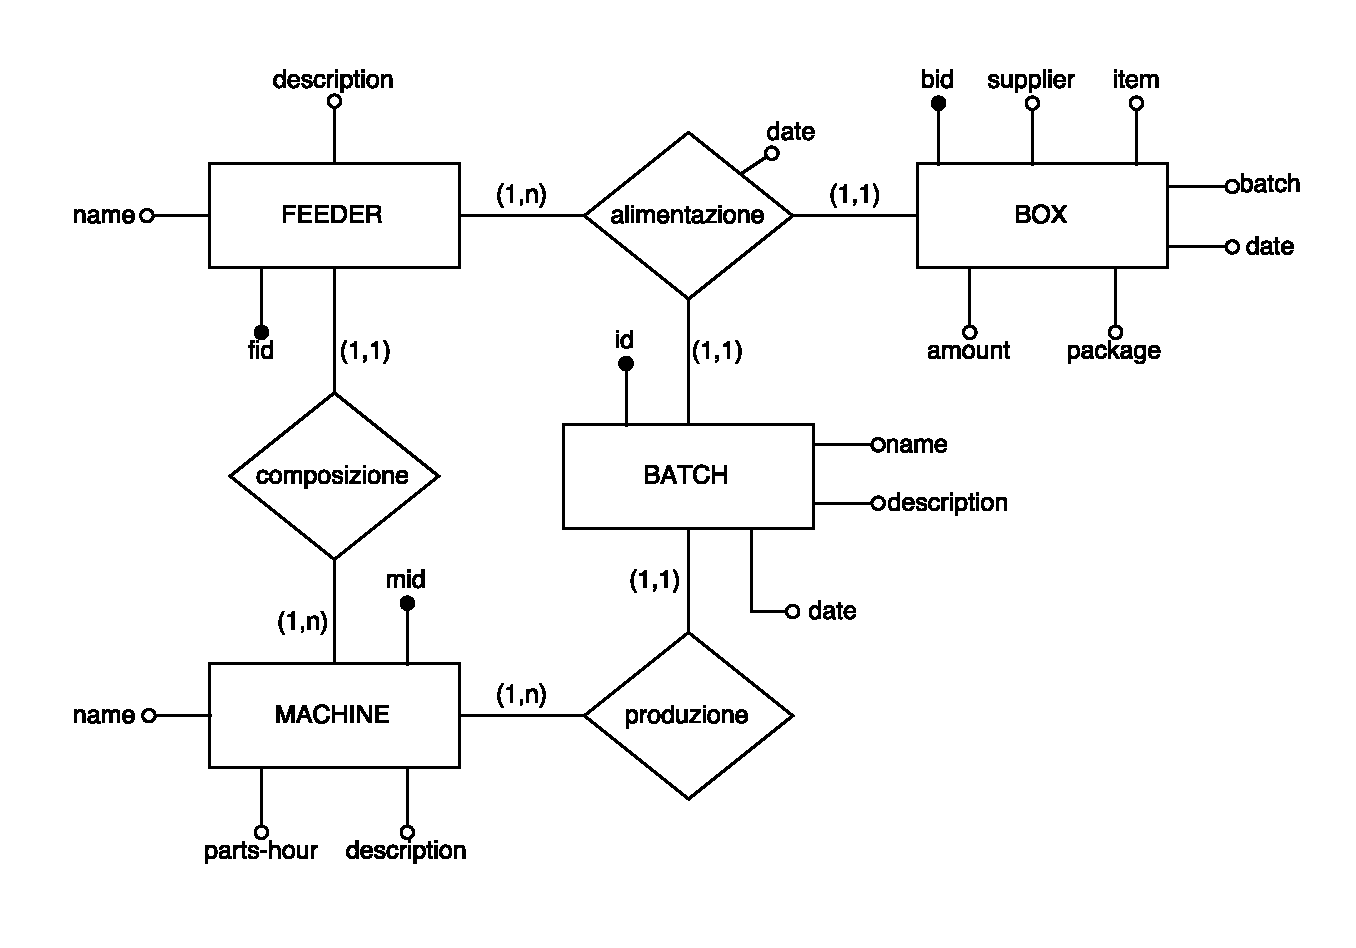
\includegraphics[scale=0.7]{modelloER}
\caption{}
\label{}
\end{figure}
\begin{table}[h!]
\centering
\begin{tabular}{| l | p{3cm} | p{3cm} | p{3cm} |}
\hline Entità & Descrizione & Attributi & Identificatore\\
\hline Machine & Macchina nella linea di produzione & mid, name, description, parts\_hour & mid\\
\hline Feeder & Alimentatore della macchina & fid, name, description & fid\\
\hline Box & Scatolone di componenti riversato nell'alimentatore & bid, supplier, item, batch, date, package, amount & bid\\
\hline Batch & Lotto di produzione & id, name, description, date & id\\
\hline
\end{tabular}
\label{tab:erentity}
\caption[Documentazione ER: entità]{Documentazione schema concettuale. Tabella delle entità}
\end{table}
\paragraph{Machine}
\begin{description}
\item[mid] codice identificativo univoco della macchina
\item[name] nome assegnato alla macchine
\item[description] nome/descrizione della macchina
\item[parts\_hour] stima della produzione oraria assumendo che ogni ciclo sia positivo e quindi non ci siano scarti
\end{description}

\paragraph{Feeder}
\begin{description}
\item[fid] codice identificativo univoco dell'alimentatore
\item[name] nome dell'alimentatore
\item[description] descrizione della macchina
\end{description}

\paragraph{Box}
\begin{description}
\item[bid] codice identificativo univoco dello scatolone
\item[supplier] fornitore del componente
\item[item] identificativo del componente
\item[batch] lotto di produzione del componente
\item[date] data di produzione del componente
\item[package] collo dello scatolone
\item[amount] numero di componenti in uno scatolone
\end{description}

\paragraph{Batch}
\begin{description}
\item[id] codice identificativo univoco del lotto di produzione
\item[nome] nome assegnato al lotto di produzione
\item[description] descrizione del lotto di produzione
\item[date] data del lotto di produzione
\end{description}

\begin{table}
\begin{tabular}{| l | p{3cm} | p{3cm} | p{3cm} |}
\hline Relazione & Descrizione & Entità coinvolte & Attributi\\
\hline Composizione & Associa un alimentatore alla sua macchina & Machine, Feeder & \\
\hline Alimentazione & Associa lo scatolone caricato al suo alimentatore per produrre il lotto& Feeder, Box, Batch & date\\
\hline Produzione & Associa alla macchina il lotto di produzione & Machine, Batch & \\
\hline
\end{tabular}
\label{tab:errelationship}
\caption[Documentazione ER: relazioni]{Documentazione schema concettuale. Tabella delle relazioni}
\end{table}
\paragraph{Alimentazione}
\begin{description}
\item[date] timestamp (data/ora) del carico componenti nell'alimentatore
\end{description}

\paragraph{Progettazione logica}
\begin{figure}
\centering
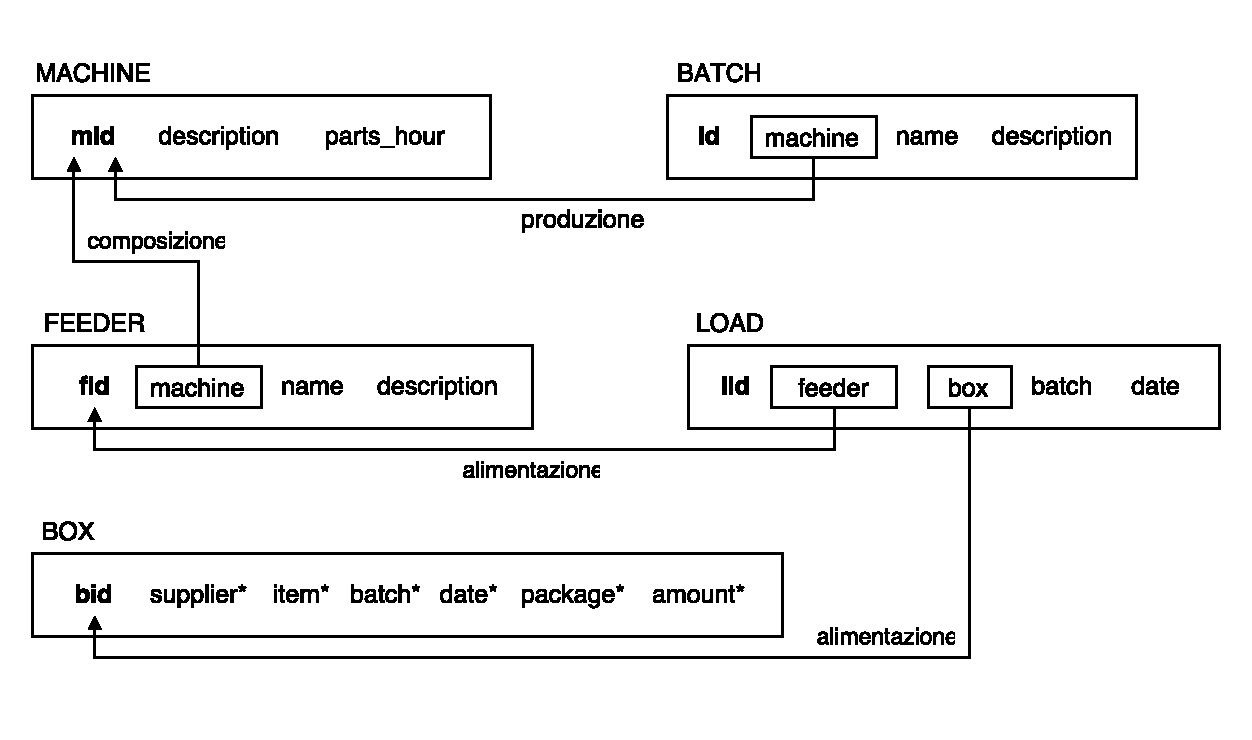
\includegraphics[scale=0.7]{modelloREL}
\caption{}
\label{}
\end{figure}

\paragraph{Relational model}
\hfill

MACHINE(\underline{mid}, name, description, parts\_hour)

FEEDER(\underline{fid}, \textit{machine}, name, description)

LOAD(\underline{lid}, \textit{feeder}, \textit{box}, \textit{batch}, date)

BOX(\underline{bid}, supplier, item, batch, date, package, amount)

BATCH(\underline{id}, \textit{machine}, name, description, date)

\paragraph{Progettazione fisica}
\begin{table}
\begin{tabular}{| l | l | l |}
  \hline Attributo & Tipo & Vincoli\\
  \hline mid & serial & primary key \\
  \hline name & varchar(32) & \\
  \hline description & varchar(256) & \\
  \hline parts\_hour & integer & \\
  \hline
\end{tabular}
\label{tab:machinetable}
\caption[Documentazione ER: relazioni]{Progettazione fisica. Tabella Machine.}
\end{table}

\begin{table}
\begin{tabular}{| l | l | l |}
  \hline Attributo & Tipo & Vincoli\\
  \hline n\_machine & smallint & not null \\
  \hline description & varchar(80) & default \lq\rq\\
  \hline usr\_desc1 & varchar(80) & default \lq\rq\\
  \hline usr\_desc2 & varchar(80) & default \lq\rq\\
  \hline teo\_parts\_hour & integer & \\
  \hline
\end{tabular}
\label{tab:machinetableimpl}
\caption[Documentazione ER: relazioni]{Progettazione fisica. Tabella Machine implementata (Machine\_desc).}
\end{table}

\begin{table}
\begin{tabular}{| l | l | l |}
  \hline Attributo & Tipo & Vincoli\\
  \hline id & serial & primary key \\
  \hline name & varchar(32) & \\
  \hline machine & integer & not null, references machine.mid \\
  \hline description & varchar(256) & \\
  \hline date & timestamp & not null, default now()\\
  \hline
\end{tabular}
\label{tab:batchtable}
\caption[Documentazione ER: relazioni]{Progettazione fisica. Tabella Batch.}
\end{table}

\begin{table}
\begin{tabular}{| l | l | l |}
  \hline Attributo & Tipo & Vincoli\\
  \hline id\_batch & serial & not null \\
  \hline n\_machine & smallint & not null \\
  \hline batch & varchar(50) & not null, default \lq\rq\\
  \hline description1 & varchar(80) & default \lq\rq\\
  \hline description2 & varchar(80) & default \lq\rq\\
  \hline description3 & varchar(80) & default \lq\rq\\
  \hline
\end{tabular}
\label{tab:batchtableimpl}
\caption[Documentazione ER: relazioni]{Progettazione fisica. Tabella Batch implementata (Batch).}
\end{table}

\begin{table}
\begin{tabular}{| l | l | l |}
  \hline Attributo & Tipo & Vincoli\\
  \hline fid & varchar(16) & primary key \\
  \hline machine & \textit{integer} (smallint) & not null, \textit{references
  machine.mid}\\
  \hline name & varchar(32) & \\
  \hline description & varchar(256) & \\
  \hline
\end{tabular}
\label{tab:feedertable}
\caption[Documentazione ER: relazioni]{Progettazione fisica. Tabella Feeder.}
\end{table}

\begin{table}
\begin{tabular}{| l | l | l |}
  \hline Attributo & Tipo & Vincoli\\
  \hline bid & varchar(128) & primary key \\
  \hline supplier & varchar(16) & \\
  \hline item & varchar(16) & \\
  \hline batch & varchar(16) & \\
  \hline date & timestamp & \\
  \hline package & varchar(16) & \\
  \hline amount & integer & \\
  \hline
\end{tabular}
\label{tab:boxtable}
\caption[Documentazione ER: relazioni]{Progettazione fisica. Tabella Box.}
\end{table}

\begin{table}
\begin{tabular}{| l | l | l |}
  \hline Attributo & Tipo & Vincoli\\
  \hline lid & serial & primary key \\
  \hline feeder & varchar(16) & not null, references feeder.feeder\_id\\
  \hline box & varchar(128) & not null, references box.bid, on delete cascade\\
  \hline batch & integer & not null, \textit{references batch.id}\\
  \hline date & timestamp & not null, default now()\\
  \hline
\end{tabular}
\label{tab:loadtable}
\caption[Documentazione ER: relazioni]{Progettazione fisica. Tabella Load.}
\end{table}
\paragraph{Adattamento e realizzazione}
\subsubsection{Dati semistrutturati per i modelli di estrazione}
\paragraph{Tecnologia XML}
\paragraph{XML Schema Definition e validazione}
\paragraph{Manipolazione e interrogazione dei dati}

\subsection{Progettazione del sistema}
\subsubsection{Comportamento del software}

\subsection{Implementazione reale}
\subsubsection{Moduli software}
\paragraph{Driver}
\paragraph{Middleware}
\paragraph{Applicativo e GUI}
\subsubsection{Limiti fisici e operativi}

\subsection{Dislocamento}
\subsubsection{Installazione}
\subsubsection{Configurazione}
\subsubsection{Avvio del servizio}
\subsubsection{Discriminazione dell'hardware}

\newpage
\subsection{Rilevamento e risoluzione degli errori}
\subsubsection{Logging degli eventi}
I moduli di questo sistema software dispongono di meccanismi di notifica degli
eventi che si occupano di registrare le principali operazioni effettuate e di
avvertire l'utente al verificarsi di problemi che ne potrebbero impedire il
normale funzionamento.

Il \textit{Log} implementato utilizza, ad eccezione di \textit{Driver}, la
classe \texttt{Logger} del package \textit{java.util.logging} \cite{jianlog} che
oltre a fornire il servizio di logging permette anche di definirne la
\textit{severità}, scegliendo una tra le costanti messe a disposizione dalla
classe \texttt{Level}. Si riportano \citesite{jdoclevel} i livelli \texttt{INFO}
per indicare eventi generici di interesse che non presuppongono un errore,
\texttt{WARNING} da usare in caso si verifichino situazioni che si separano dal
normale flusso di esecuzione e necessitano di essere gestite, \texttt{SEVERE}
per gravi problemi che potrebbero ostacolare il normale funzionamento,
\texttt{OFF} che disabilita totalmente i messaggi di log e \texttt{ALL} per
consentire ad ogni evento di essere registrato indipendentemente dal suo livello.

Data un'istanza di \texttt{Logger} definita o recuperata con il metodo statico
\texttt{getLogger()} sono processati solo i messaggi il cui livello di
severità è maggiore o uguale a quello definito per l'istanza stessa con il
metodo \texttt{setLevel()}.

Severità e testo del messaggio dunque sono parametri da indicare per ogni
\texttt{LogRecord} quando di registra un evento con il metodo \texttt{log()};
i metodi alternativi \texttt{info()}, \texttt{warning()}, \texttt{severe()} non
necessitano del livello di severità.

\vspace{5mm}

Il servizio di logging per il modulo \textit{Driver} è implementato con la
procedura \texttt{logger()} definita come in listato \ref{lst:loggerdef} e
invocata dai thread in esecuzione per stampare i messaggi sul canale
\textit{stdin}.

\vspace{5mm}

\lstinputlisting[caption={Definizione procedura logger().},
label={lst:loggerdef}]{./code/logger.c}

Diversamente dal package di Java, il linguaggio C non dispone dei livelli di
severità. Questa caratteristica è simulata con la variabile globale
\texttt{tolog} inizializzata dal processo padre e acceduta in lettura dai thread
figli così da condizionare il comportamento della procedura. I valori possibili
per \texttt{tolog} sono: \texttt{0} per disattivare il servizio di log,
\texttt{1} per attivarlo.

\vspace{5mm}
 
Il logging degli eventi è inattivo di default tutti i moduli. La sua attivazione
richiede di specificare l'opzione \texttt{-d} al momento dell'esecuzione del software.
\subsubsection{Aggregatore}
bla
\newpage

\section{valutazione della soluzione}

\subsection{collaudo/test/risposta del sistema}

\subsection{dati in appoggio}


\section{Conclusioni}
\label{sec:concl}

\subsection{Risultati ottenuti}

\subsection{Sviluppi futuri}

\subsection{Ringraziamenti}

\appendix
\input{./sections/appendice.tex}
\cite{ahu61}

\newpage
\bibliography{./sections/bibliografia}
\bibliographystyle{plain}

\end{document}